\chapter{Results of experiments with \nqp}
\label{app:nqp}
\textit{In this appendix results values of experiments with \nqp{} are presented.}
\vfill
\newpage

Column labels:
\begin{itemize}
\item \texttt{Sequential}: Experiment using one core.
\item \texttt{Parallel}: Experiment using 40 cores without communication.
\item \texttt{K \% / com. 1-1}: Experiment with $K$\% of communicating solvers ($\tfrac{K}{2}$\% of sender solvers, and $\tfrac{K}{2}$\% of receiver solvers) using communication \textit{one~to~one}, and $100-K$\% of non-communicating solvers.
\item \texttt{K \% / com. 1-N}: Experiment with $K$\% of communicating solvers ($\tfrac{K}{2}$\% of sender solvers, and $\tfrac{K}{2}$\% of receiver solvers) using communication \textit{one~to~N}, and $100-K$\% of non-communicating solvers.
\item \texttt{Time}: Time in milliseconds. 
\item \texttt{Iter.}: Number of iterations.
\end{itemize}

Color caption:
\begin{itemize}
\item \gracias{Values in red color}: A receiver solver was the winner, finding the solution thanks to the received information.
\item \receiver{Values in dark red color}: A receiver solver was the winner, finding the solution without tacking into account the received information.
\item \sender{Values in blue color}: A sender solver was the winner.
\item \nocomm{Values in black color}: A non-communicating solver was the winner.
\end{itemize}

%\noindent\rule[2pt]{\textwidth}{0.8pt}

\clearpage
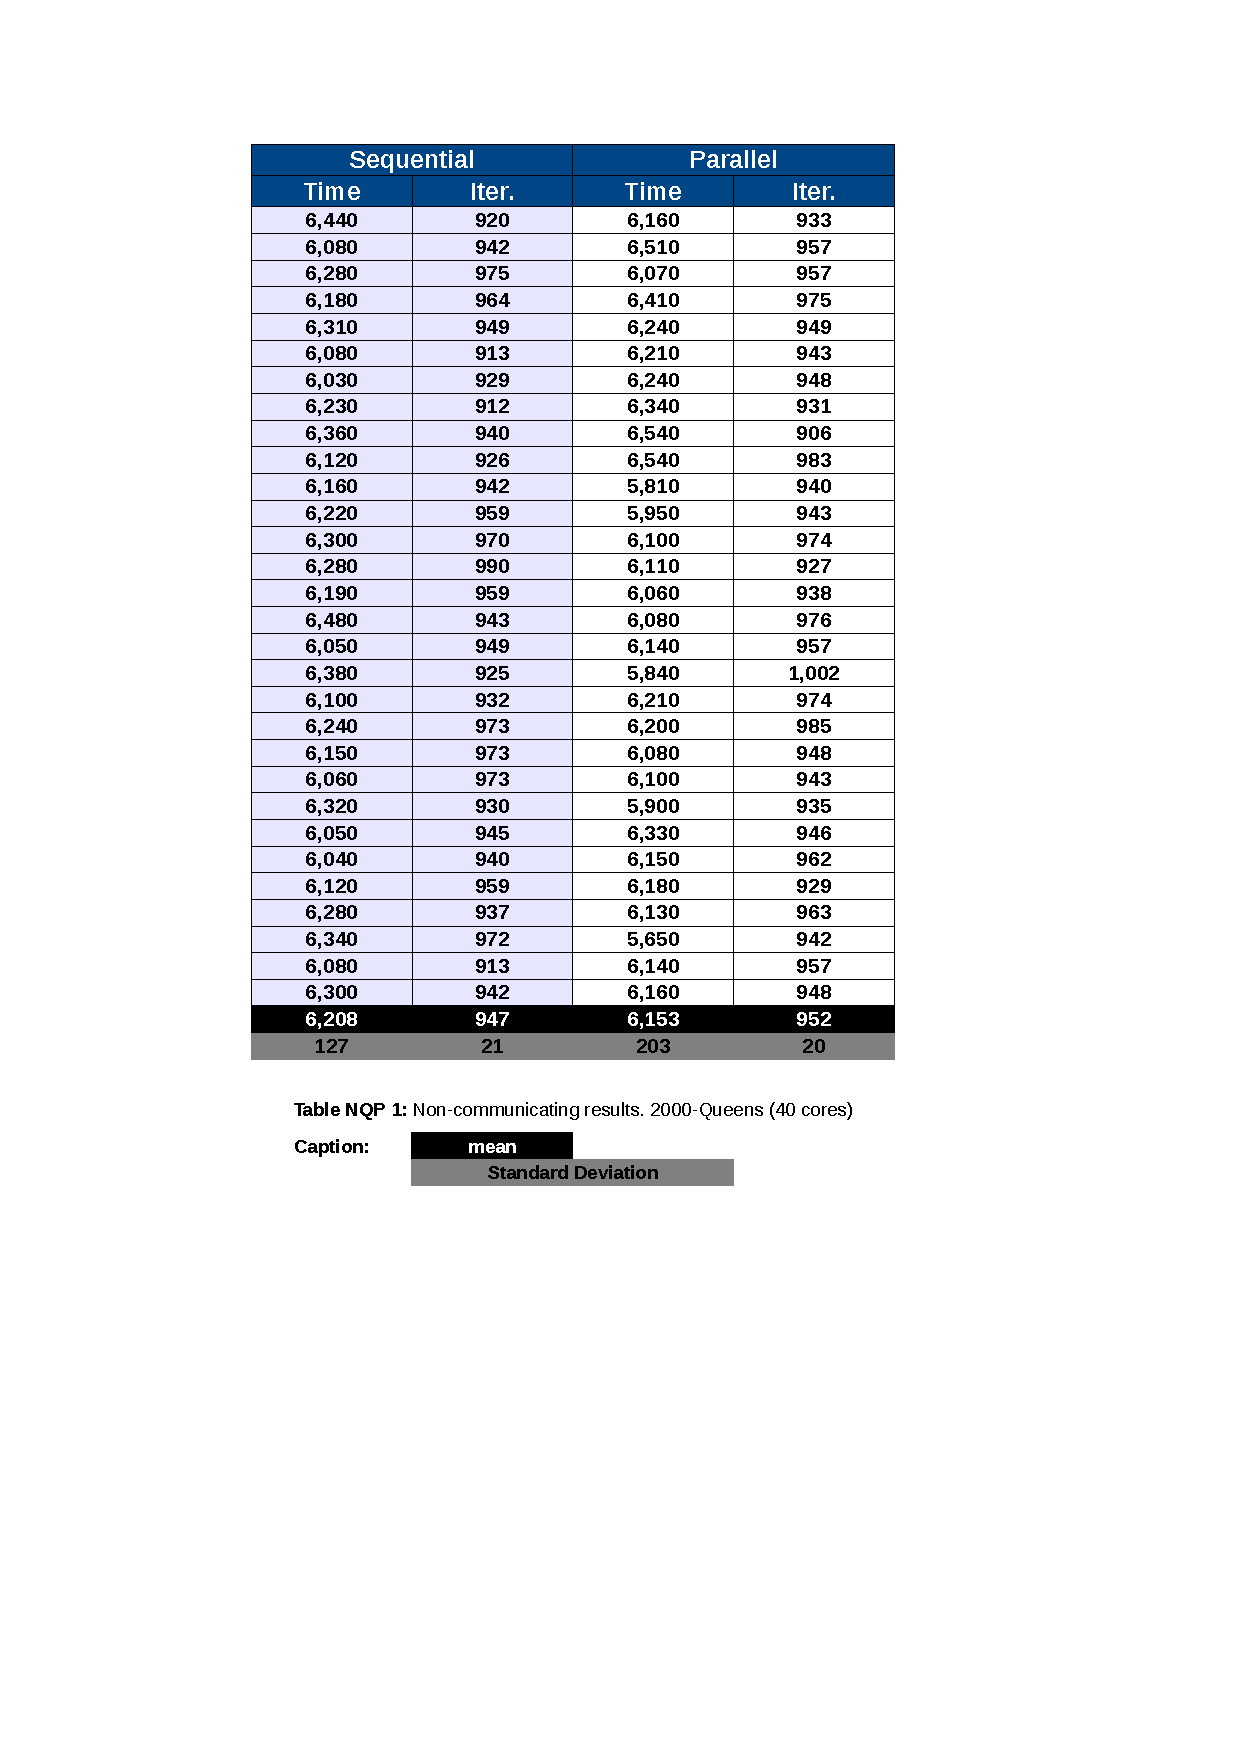
\includepdf[pages=-]{appres//res_nqueens.pdf}